% This file was created by matlab2tikz.
%
\definecolor{mycolor1}{rgb}{0.89412,0.10196,0.10980}%
\definecolor{mycolor2}{rgb}{0.21569,0.49412,0.72157}%
%
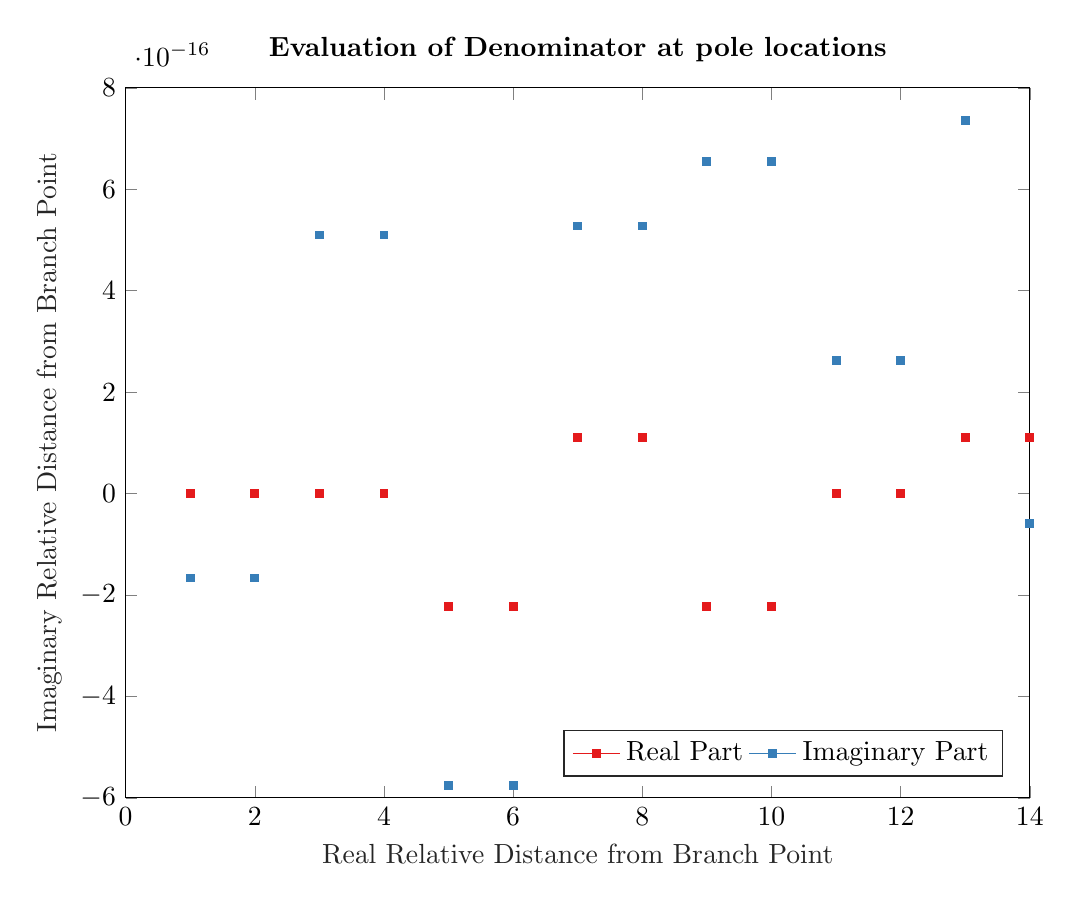
\begin{tikzpicture}

\begin{axis}[%
width=4.521in,
height=3.55in,
at={(0.758in,0.497in)},
scale only axis,
xmin=0,
xmax=14,
xlabel style={font=\color{white!15!black}},
xlabel={$\textrm{Real Relative Distance from Branch Point}$},
ymin=-6e-16,
ymax=8e-16,
ylabel style={font=\color{white!15!black}},
ylabel={$\textrm{Imaginary Relative Distance from Branch Point}$},
axis background/.style={fill=white},
title style={font=\bfseries},
title={Evaluation of Denominator at pole locations},
legend style={at={(0.97,0.03)}, anchor=south east, legend columns=2, legend cell align=left, align=left, draw=white!15!black}
]
\addplot [color=mycolor1, draw=none, mark size=1.4pt, mark=square*, mark options={solid, fill=mycolor1, mycolor1}]
  table[row sep=crcr]{%
1	0\\
2	0\\
3	0\\
4	0\\
5	-2.22044604925031e-16\\
6	-2.22044604925031e-16\\
7	1.11022302462516e-16\\
8	1.11022302462516e-16\\
9	-2.22044604925031e-16\\
10	-2.22044604925031e-16\\
11	0\\
12	0\\
13	1.11022302462516e-16\\
14	1.11022302462516e-16\\
};
\addlegendentry{Real Part}

\addplot [color=mycolor2, draw=none, mark size=1.4pt, mark=square*, mark options={solid, fill=mycolor2, mycolor2}]
  table[row sep=crcr]{%
1	-1.66533453693773e-16\\
2	-1.66533453693773e-16\\
3	5.10008701937181e-16\\
4	5.10008701937181e-16\\
5	-5.74843991851814e-16\\
6	-5.74843991851814e-16\\
7	5.27586329658603e-16\\
8	5.27586329658603e-16\\
9	6.54990249321016e-16\\
10	6.54990249321016e-16\\
11	2.62843640895429e-16\\
12	2.62843640895429e-16\\
13	7.34830821367669e-16\\
14	-5.86498977849625e-17\\
};
\addlegendentry{Imaginary Part}

\end{axis}
\end{tikzpicture}%